\section{Experimental Evaluation}

In this section we detail the results obtained when testing our actuation techniques. As CPU power consumption is the major contributor to overall server power, for time reasons, we focus our experiments on the CPU subsystem.
\subsection{Main test}

To obtain some results in the next actuation techniques, a script to launch all the benchmarks has been executed in the server. This script executes all the selected benchmarks through all the possible energy-consumption configurations in order to obtain some metrics.

\begin{lstlisting}[language=Bash]
for frecuency in Frecuencies[@]; do
    change_cpu_freq -all
    sleep 1m
    for benchmark in Benchmarks[@]; do
        for numberCPUs in Cpus[@]; do
            disable_cpu <numberCPUs>
            for numberCopies in Copies[@]; do
                - Execute the Benchmark -
                sleep 5m
            done
        done
    done
done
\end{lstlisting}

As explained in chapter 4, 128 Benchmark-Configuration pairs were executed and the results will be analyzed in the following section.

\subsection{CPU and Memory intensive benchmarks}

Apart from analyzing how power consumption is reduced, it is also important to be able to detect when a benchmark is CPU or memory intensive. To do so, some counters help us.

As expected, Perlbench and Calculix have more "instructions per cycle" (IPC) than Mcf and Lbm. This is because memory intensive benchmarks have much more "Last Level Cache Misses" (LLC\_Misses). This issue makes the processor work slower because it has to wait until the thread access to the main memory to recover the data needed.

As we are running several copies of sequential benchmarks, as long as there is no contention, IPC and LLC can be used to cluster benchmarks into various categories. Moreover, this two metrics are not affected by the processor frequency. Thus, IPC and LLC depend on the benchmark being executed. For that reason, when a new workload is executed, its type can be easily detected and this can be an interesting point to start the design of a new policy.

Next figure shows the average IPC and LLC\_misses.

\begin{table}[H]
\begin{center}
\begin{tabular}{p{4cm} p{3cm} p{3cm}}
  \bf &  IPC & LLC Misses \\
  \bf Pearlbench & 1.76 & 3.68 $\cdot {10}^{8}$ \\
  \bf Calculix & 2.49 & 2.05 $\cdot {10}^{8}$\\
  \\
  \bf Lbm & 1.18 & 2.22 $\cdot {10}^{9}$\\
  \bf Mcf & 0.39 & 6.43 $\cdot {10}^{8}$\\
\end{tabular}
\end{center}
\caption{IPC and LLC misses for each benchmark}
\label{tab:ipcllc}
\end{table}

\begin{figure}[H]
\begin{center}
\includegraphics[scale= 0.80]{llcipc} % Podría poner[width=\linewidth]
\caption{IPC and LLC misses for each benchmark}
\label{fig:llcipc} %Establece una etiqueta para la figura
\end{center}
\end{figure}


\subsection{DVFS}

Now, DVFS consequences in power consumption will be analyzed. For the next figures, the value of CPU total consumption is used to compare all the benchmarks. It would be better to compare the Dynamic consumption of the cpu, but the values are not so accurate. The sensor that is installed in the Decathlete to measure the consumption of the server has a resolution of 4W. As some of the dynamic values are below 4W, this values will not be used in this comparison.

In some data centers there is a need to put a cap on maximum power, to ensure that the facility does not exceed the maximum power budget. In such cases, we may benefit from lowering frequency to save power. However, among the various configurations, we need to chose one that reduces. Based on this results, we could develop policies to set the frequency of servers depending on the particular workload to be executed.

To calculate the total consumption of the CPU, we have subtract the power consumption of the disks, memories and fans from the value of total consumption of the server. All this values have been obtained using Graphite, so they are all experiment results. The X axis contains each benchmark, while the Y axis shows the power consumption.

\begin{comment}
The X axis represents, using a code, each benchmark. The code can be interpreted this way:

Part1\_Part2\_Part3
\begin{itemize}
\item [$-$] Part1: This is the name of the type of the benchmark. As it was detailed in a previous section, there are four benchmarks: Perlbench, Calculix, Mcf and Lbm.
\item [$-$] Part2: This is the number of threads enabled. Possible values are 1, 3, 6 and 12
\item [$-$] Part3: This is the number of copies of the same benchmark executed at the same time. Possible values depend on the number of threads enabled.
\end{itemize}
\end{comment}

Figure \ref{fig:potenciaFreq} shows how power consumption depends on the frequency.


\begin{figure}[H]
\begin{center}
\includegraphics[scale= 0.65]{compPower2} % Podría poner[width=\linewidth]
\caption{Power consumption in Watts depending on the frequency}
\label{fig:potenciaFreq} %Establece una etiqueta para la figura
\end{center}
\end{figure}

Analyzing the results, it can be seen that power depends on the frequency. For the same benchmark, savings of almost 25\% can be achieved reducing the frequency from 2001MHz to 1200MHz. Of course, as power does not depend on the time elapsed, benchmarks cannot be only compared this way. For this reason, in Figure \ref{fig:edpFreq} the EDP of each benchmark is shown. To calculate the EDP, power has been multiplied by the second power of the time, which has been obtained thanks to a log saved during the execution of the script.

\begin{figure}[H]
\begin{center}
\includegraphics[scale= 0.6]{edp_Freq5} % Podría poner[width=\linewidth]
\caption{EDP of each benchmark depending on the Frequency}
\label{fig:edpFreq} %Establece una etiqueta para la figura
\end{center}
\end{figure}

In this Figure, changes can be seen when we consider the contribution of time to the metric. Despite the power consumption is lower, the time elapsed is higher so the EDP recommends to use the highest frequency. Energy plot is not shown given that its shape is similar to the EDP one, so it is not necessary.

According to the data obtained, it is experimentally demonstrated that the choice of the most suitable frequency depends on the aim to achieve. If the goal is to minimize the power consumption - reducing the power consumption peaks - it is better to reduce the frequency of the processor. If the goal is to maximize the performance and, therefore, minimize the energy consumption and the EDP, the most suitable solution is to run at higher frequencies.

Despite this level of detail cannot be represented in the plot, the gap between 2001MHz and the others is higher than the rest. The reason is that 2001Mhz is the Turbo Boost frequency. As it was explained in the DVFS section, at this frequency the processor has to do its best and this maximizes the contribution to the CPU power consumption.


It can be seen also in Figure \ref{fig:edpFreq} that not all the Benchmarks vary the same when the frequency changes. Those which are cpu intensive have a higher variation in it EDP. This is because cpu benchmarks depends only on how fast can the processor calculate. When the frequency is high the EDP is lower. However, in mcf and lbm benchmarks, the bottleneck is not for the processor, but for the time elapsed accessing to the main memory. For that reason, the EDP does not vary at all in them.


\subsection{Disabling Threads}

%%Aquí las cosas de comparar idle.

\emph{Analysis of the idle consumption}

Disabling threads has also given interesting results. First of all, it has been analyzed if disabling them could achieve savings in power consumption. As it is shown in Figure \ref{fig:cpuGraf}, which is a capture of Graphite, mean power consumption is constant when the number of threads changes.

In this capture, the same process as in the other tests has been followed. The server has been configured for 5 minutes in all the power consumption possible configurations. The plot represents the total consumption of the server in the Y axis, while the X axis represents the time.

\begin{figure}[H]
\begin{center}
\includegraphics[scale= 0.52]{grafIDLE} % Podría poner[width=\linewidth]
\caption{Total server consumption depending on frequency and threads enabled}
\label{fig:cpuGraf} %Establece una etiqueta para la figura
\end{center}
\end{figure}

This means that even though we are disabling threads in user space, the change is not being implemented in lower levels, i.e. it is not directly supported by the Intel CPU drivers. In this sense, we observe no benefits in terms of power when disabling threads in idle load.

\ \\ 

\emph{Analysis of the consumption of a workload}
%%Aquí las cosas de comparar benchmarks

Apart from the test above, in which no benchmark was running, so as the idle power was similar to CPU and proportional to the total server power consumption, another test has been run. Now, the same test as in the DVFS section will be analyzed.

Despite we have not been able to turn off CPUs, threads have been disabled. This give us the opportunity to study the performance depending on the number of threads.

In Figure \ref{fig:timeProc} the performance of each benchmark will be analyzed. The time elapsed in each benchmark is represented in the Y axis and the X axis has each benchmark. 

\begin{comment}The benchmark code must be analyzed in the same way:

Part1\_Part2
\begin{itemize}
\item [$-$] Part1: This is the name of the type of the benchmark. As it was detailed in a previous section, there are four benchmarks: Perlbench, Calculix, Mcf and Lbm.
\item [$-$] Part2: This is the frequency at which the processor runs for this benchmark.
\end{itemize}
\end{comment}

\begin{figure}[H]
\begin{center}
\includegraphics[scale= 0.6]{timeProc3} % Podría poner[width=\linewidth]
\caption{Time spent in each benchmark}
\label{fig:timeProc} %Establece una etiqueta para la figura
\end{center}
\end{figure}

As it can been seen in this figure, there are two different performances when disabling threads. When using only one core for one thread, the time elapsed grows. This is caused by two reasons: 

\begin{itemize}
\item [$-$] First, when using just one thread, all the processes must be executed in the same thread. This means that all OS processes have to share the processor resources with the benchmark. This issue caps the performance. When more that 1 thread is enabled, one of them can be exclusively used for the benchmark.

\item [$-$] Second, Hyper-threading which is the Intel's proprietary simultaneous multithreading (SMT) implementation. This technology makes the processor compute faster. 
\end{itemize}

The main function of hyper-threading is to increase the number of independent instructions in the pipeline; it takes advantage of superscalar architecture, in which multiple instructions operate on separate data in parallel. In addition, two or more processes can use the same resources: if resources for one process are not available, then another process can continue if its resources are available. This enables the server to make a better performance when using several threads.

\ 

CPU power consumption seems to remain the same. Figure \ref{fig:powerProc} represents the cpu total power consumption in Y axis for each Benchmark in X axis depending on the number con threads enabled. 

\begin{figure}[H]
\begin{center}
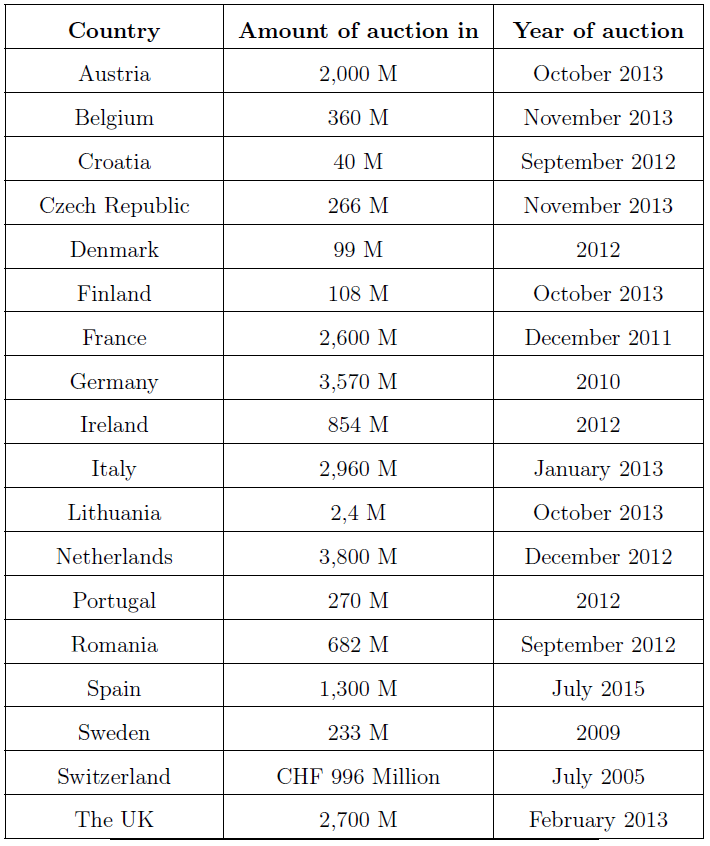
\includegraphics[scale= 0.6]{Screenshot_1} % Podría poner[width=\linewidth]
\caption{CPU power consumption depending on frequency and threads enabled}
\label{fig:powerProc} %Establece una etiqueta para la figura
\end{center}
\end{figure}

All the plots have the same shape. The "1 Thread Plot" has lower CPU power consumption. This reduction is not more than 4W which is the sensor resolution, so no assurance may be given.

This difference is because the total consumption of the server remains the same, but the consumption of fans and memories increases 1-2W. Figure \ref{fig:powerProcTotal} represents the total consumption of the server which we can see that is the same for any number of threads enabled.

\begin{figure}[H]
\begin{center}
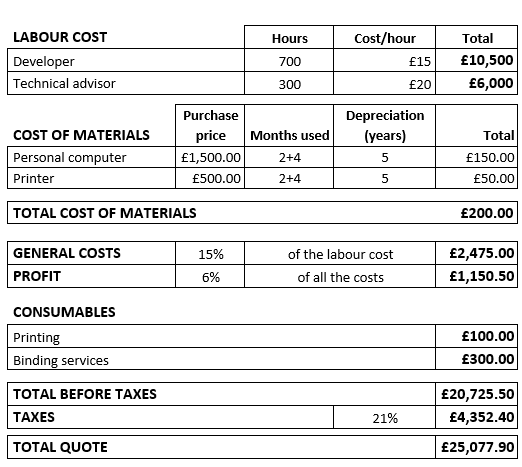
\includegraphics[scale= 0.6]{Screenshot_2} % Podría poner[width=\linewidth]
\caption{Total power consumption depending on frequency and Threads enabled}
\label{fig:powerProcTotal} %Establece una etiqueta para la figura
\end{center}
\end{figure}

Finally, all this study would have given more results if intel-pstate driver was enabled to be configured by the user. The newest Intel servers have this driver that allows the OS to manage the number of cores that are turned on and off depending of the workload.

\subsection{Analysis of tentative policies}

In this section, a comparison between DVFS and disabling threads will be given. The point is to study which actuation technique is better to apply when consumption reduction is needed.

First of all, if the need is to achieve a peak power consumption reduction, given that disabling threads does not reduce the power consumption, the only way is reducing the frequency of the processor. Reducing the frequency, the processor computes slower and consumes less power. Figure \ref{fig:compPower} represents the CPU total consumption depending on the frequency.

\begin{figure}[H]
\begin{center}
\includegraphics[scale= 0.7]{compPower2} % Podría poner[width=\linewidth]
\caption{CPU power consumption depending on frequency}
\label{fig:compPower} %Establece una etiqueta para la figura
\end{center}
\end{figure}


When energy consumption reduction is the aim, the choice is not as simple as power. We have two actuation techniques that are orthogonal between them and the best solution is not just incrementing one of them. Table \ref{tab:energComp} is an example of the consumption of a benchmark - perlbench - depending on the frequency and the number of threads enabled. Despite this table shows a particular example, this reasoning can be applied to all benchmarks.

\begin{table}[H]
\begin{center}
\begin{tabular}{ccccc}
  \bf Perlbench &  1200MHz & 1500MHz & 1700MHz & 2001MHz \\
  \bf 1 Thread &  7.5 $\cdot {10}^{4}$ & 5.6 $\cdot {10}^{4}$ & 5.1 $\cdot {10}^{4}$ & 3.6 $\cdot {10}^{4}$ \\
  \bf 3 Threads & 5.3 $\cdot {10}^{4}$ & 4.5 $\cdot {10}^{4}$ & 4.1 $\cdot {10}^{4}$ & 3.2 $\cdot {10}^{4}$ \\
  \bf 6 Threads & 5.3 $\cdot {10}^{4}$ & 4.4 $\cdot {10}^{4}$ & 4.0 $\cdot {10}^{4}$ & 3.3 $\cdot {10}^{4}$ \\
  \bf 12 Threads & 5.4 $\cdot {10}^{4}$ & 4.4 $\cdot {10}^{4}$ & 4.1 $\cdot {10}^{4}$ & 3.3 $\cdot {10}^{4}$ \\

\end{tabular}
\end{center}
\caption{CPU energy consumption of 1 copy of Perlbench depending on Frequency and number of threads enabled }
\label{tab:energComp}
\end{table}

As it can be seen in the table, if we are executing one copy of Perlbench with just one core and 1200Mhz, and we need to reduce the energy consumed, the first step would be increasing the number of threads enabled for this benchmark to 3 threads.

Then there is no more reduction for enabling more threads - this is because more than 2 threads does not reduce the time elapsed. Now, it would be necessary to increase the frequency using DVFS.

Increasing frequency reduces energy consumption, but it should be the opposite. This is because we are always using the Total CPU Consumption data. This data contains the contribution of the IDLE consumption, which is large and constant, and it is calculated depending on the time elapsed in the benchmark. 

When only the dynamic CPU power consumption is compared, energy consumption has a growth of consumption trend with the frequency. The issue is that the power measured is lower than the sensor resolution, so values are just indicative. 
%\begin{comment}
Table \ref{tab:energCompdyn} shows this information for the same benchmark.

\begin{table}[H]
\begin{center}
\begin{tabular}{ccccc}
  \bf Perlbench &  1200MHz & 1500MHz & 1700MHz & 2001MHz \\
  \bf 1 Thread &  2.7 $\cdot {10}^{3}$ & 1.7 $\cdot {10}^{3}$ & 3.7 $\cdot {10}^{3}$ & 5.4 $\cdot {10}^{3}$ \\
  \bf 3 Threads &  1.2 $\cdot {10}^{3}$ & 2.8 $\cdot {10}^{3}$ & 4.1 $\cdot {10}^{3}$ & 5.6 $\cdot {10}^{3}$ \\
  \bf 6 Threads & 2.9 $\cdot {10}^{3}$ & 3.1 $\cdot {10}^{3}$ & 3.8 $\cdot {10}^{3}$ & 5.8 $\cdot {10}^{3}$ \\
  \bf 12 Threads &  2.6 $\cdot {10}^{3}$ & 2.7 $\cdot {10}^{3}$ & 4.7 $\cdot {10}^{3}$ & 5.9 $\cdot {10}^{3}$ \\

\end{tabular}
\end{center}
\caption{Dynamic CPU energy consumption of 1 copy of Perlbench depending on Frequency and number of threads enabled }
\label{tab:energCompdyn}
\end{table}
%\end{comment}

These are the results that have been obtained from the study of the Decathlete server in this thesis. In the next chapter, the most important conclusions and the proposed future lines of work will be detailed.